\documentclass[norsk,a4paper,12 pt]{article}
\usepackage{graphicx}
\graphicspath{ {images/} }
% Setter orddelingsregler for norsk (se opsjon "norsk" over)
\usepackage{babel}
% Setter UTF-8 tegnsett for latex (et passende utvalg fra Unicode for norsk)
\usepackage{ucs}
\usepackage[utf8x]{inputenc}
\usepackage[T1]{fontenc}
\PreloadUnicodePage{0}
% Håndterer mellomrom på en smidig (og automatisk) måte.
\usepackage{xspace}
% Gjør lenker (også internt i dokumentet) klikkbare
\usepackage{hyperref}
% God formatering av URL
\usepackage{url}
% Gjør farger tilgjengelig, feks fargede bokstaver og strektegninger
\usepackage{color}
% Kommandoer for å integrere bilder i teksten
\usepackage{graphicx}
% Justering av margene (mindre enn standard oppsett)
\usepackage[hmargin=3.5cm,vmargin=2.7cm]{geometry} 


% Tittel, forfatter(e)
\title{Obligatorisk oppgave 2 inf112}
\author{cli022 qaf006 afo035}



\begin{document}
% Legger tittelen først i dokumentet
\maketitle
% Lager en innholdsfortegnelse - kommentert ut
% \tableofcontents
% Starten på selve teskten

\section{Innledning}

For den andre obligatoriske oppgaven har gruppen valgt å lage et tower defence spill som implementerer vær og tid fra www.yr.no.
Tower defence er en subsjanger av strategispill hvor målet er å forsvare spillerens område eller hovedbygning. 
Spilleren bygger som oftest tårn i smarte lokasjoner for å gjøre mest mulig skade mot innkommende fiender.
Tower defence spill er ofte veldig strategisk og har flere perspektiv til strategi, som posisjon, liv og penger.
Siden vi tar inn åpne vær og tid data fra www.yr.no, finnes det enda et perspektiv hvor fiendenes adferd vil bli påvirket av været. 
Hvis det er kaldt og is, så vil fiendene skli raskere og vil heller ikke gå i en rett linje mot hovedtårnet, hvis det er varmt så vil fiendene gå saktere, men samtidig tåle mer.
Vårt tower defence spill er også basert på utelivet, tårnene som bygges av spilleren er utesteder som skyter alkohol mot studenter.
Spilleren vil få mer penger til å bygge større utesteder som kan skyter mer alkohol og gjør mer skade hvis spilleren overlever de forskjellige rundene.
Hvis fiendene kommer seg igjennom til hoved tårnet så vil spilleren miste liv, og hvis fiendene ødelegger hovedtårnet så er spillet ferdig.
Banene vil være tilfeldig genererte og kan ha forskjellig vanskelighetsgrad.
Spillet vårt heter bar to bar tower defence.
Spillets baner vil være modellerte bilder fra forskjellige steder som for eksempel Bergens brygge eller Stavangers utested stripe. Banene vil ha lik oppbygging på vanskelighetsgraden, men vil være forskjellig estetisk.


\section{Spill manual}


\subsection{Målgruppe}


Målgruppen for vårt spill er studenter og generelt sett folk som liker å spille tower defence spill.
Tower defence spill på tablet og telefon er et veldig effektivt tidsfordriv i tillegg til at spillet baserer seg på utelivsbransjen, så derfor vil spillet appellere til de fleste som liker spill.
\subsection{Spillrunde}


Hver spillrunde vil økes siden mer fiender kommer, første runde tar kanskje 20-30 sekunder, så vil fiendene komme på nytt og bevege seg mot hoved tårnet, hver gang fiendene kommer på nytt er det mer av de slik at vanskelighetsgraden øker. Så spillrundene tar mer tid og bygger på hverandre. Det vil være mulig å lagre spillet og fortsette senere hvis spilleren ønsker, men man kan kun lagre spillet i mellom rundene. Mellom hver spillrunde så må spilleren trykke på start for å gå videre. Dette er slik at spilleren trenger å ha tid for å plassere utesteder strategisk for å skyte alkohol på fiendene!
\subsection{En-spiller spill}


Spillet er et en-spiller spill hvor det er menneske mot spillsystemet. 
Flere spillere kan spille samtidig mot sin egen datamaskin, men ikke samarbeide. Det vil være en high score liste på nettet hvor spillere kan sammenligne sitt resultat med hverandre.Det vil være valgfritt å dele sitt resultat med verden.

\section{Brukerfortellinger}


Som spiller ønsker jeg å tjene penger per runde, får å kunne 
kjøpe/oppgradere tårn.
\begin{itemize}
\item Spilleren skal motta en sum penger etter hver runde. (funksjonell)
    
\item Denne summen skal stige per runde, da belønningen skal stå i stil med rundens vanskelighetsgrad. (ikke-funksjonell)
\end{itemize}
Som spiller ønsker jeg å plassere ut tårn (nattklubber) for å kunne bekjempe fiender.
\begin{itemize}
\item Spilleren skal kunne kjøpe og plassere ut tårn på kartet. (funksjonell)

\item Dette vil ikke være mulig om spilleren ikke har nok penger. (ikke-funksjonell)

\item Spilleren skal ikke kunne plassere tårn i løypen. (ikke-funksjonell)

\item Prisen vil variere avhengig av hvilket tårn spilleren ønsker å kjøpe. (ikke-funksjonell)
\end{itemize}
Som spiller ønsker jeg å oppgradere tårn (nattklubber) for å gjøre mer skade.
\begin{itemize}
\item Spilleren skal kunne oppgradere sine tårn. (funksjonell)
\item Dette vil ikke være mulig om spilleren ikke har nok penger. (ikke-funksjonell)
\item Prisen vil stige hver gang spilleren oppgraderer et tårn, slik at det blir 
dyrere å oppgradere fra nivå to til tre, enn nivå en til to. (ikke-funksjonell)
\item Tårnet skal gjøre mer skade avhengig av hvilket nivå det er på. (ikke-funksjonell)
\end{itemize}
Som spiller ønsker jeg å kunne lagre, for å ikke miste fremgang. 
\begin{itemize}
\item Spilleren skal kunne lagre eventuell fremgang. (funksjonell)
\item Dette skal kun være mulig MELLOM hver runde, ikke i løpet av en runde. (ikke-funksjonell)
\end{itemize}

Som spiller ønsker jeg å kunne laste inn tidligere spill
\begin{itemize}

\item Spiller skal kunne laste inn tidligere lagret fremgang. (funksjonell)
\end{itemize}
Som spiller ønsker jeg en stigende vanskelighetsgrad per runde, for å stadig bli utfordret.
\begin{itemize}
\item Vanskelighetsgraden skal øke per runde. (funksjonell)

\item Antall fiender skal øke per runde. (ikke-funksjonell)

\item Tøffere fiender skal dukke opp utover spillets runder. (ikke-funksjonell)
\end{itemize}
Som spiller ønsker jeg at været i Bergen, skal reflekteres i spillet.
\begin{itemize}

\item Spillet skal hente åpne værdata fra yr.no. (funksjonell)

\item Været i spillet skal stå i samsvar med været i Bergen (funksjonell)

\item Hver dag i yr.no sin langtidsvarsel skal representeres av en runde i spillet.(ikke-funksjonell)

\item Dersom antall runder overstiger antall tilgjengelig dager med værvarsel, skal dagene starte på ny, slik at påfallende runde vil representere dag 1. (ikke-funksjonell)

\end{itemize}
Som spiller ønsker jeg at været påvirker fiendenes adferd slik at spillopplevelesen blir mer variert.
\begin{itemize}
\item Fiendenes oppførsel skal påvirkes av været. (funksjonell)

\end{itemize}

\section{Bruksmønster}


\subsection{ happy path:}

 (Spiller er aktør, Spillet er systemet)


(a) Spiller starter Spillet

(b) Spiller får generert kart og det regner

(c)Spiller starter med penger og liv, penger brukes for å bygge tårn og velger hvor tårn plasseres

(d) Spiller trykker start for ny runde

(e)Spillet genererer fiender som sklir rundt og sender de mot hoved tårnet, Spillet har kontroll over penger og liv

(f)Spiller skyter alkohol med tårnene mot fiendene og dreper de

(g)Spillet viser at runden er ferdig og oppgraderer penger og liv statusen til Spiller

(h)Spiller kan bruke pengene til å oppgradere tårn

(i) Spiller trykker start for ny runde går tilbake til (e) 



\subsection{ alternative plot:}

Hvis spillet ikke starter (Spiller er aktør, spillet er systemet)


(a) Spiller starter Spillet

(b) Spiller får generert kart og det er fint vær

(c)Spiller starter med penger og liv, penger brukes for å bygge tårn og velger hvor tårn plasseres

(d) Spiller trykker start for ny runde

(e) Spillet starter ikke

(f) Spiller får valget om å prøve på nytt eller avslutte spillet

(g)Spiller trykker start for ny runde



\subsection{ alternative plot 2:}

Hvis spilleren ikke overlever runden( Spiller er aktør, Spillet systemet)



a) Spiller starter Spillet

(b) Spiller får generert kart og det snør

(c)Spiller starter med penger og liv, penger brukes for å bygge tårn og velger hvor tårn plasseres

(d) Spiller trykker start for ny runde

(e)Spillet genererer fiender som sklir og sender de mot hoved tårnet, Spillet har kontroll over penger og liv

(f)Spiller skyter alkohol med tårnene mot fiendene, men fiendene slipper igjennom

(g)Spiller mister liv og dør 

(i) Spiller får opp high score liste av Systemet

(j) Spiller trykker start for å spille runden på nytt

\section{UML diagram}

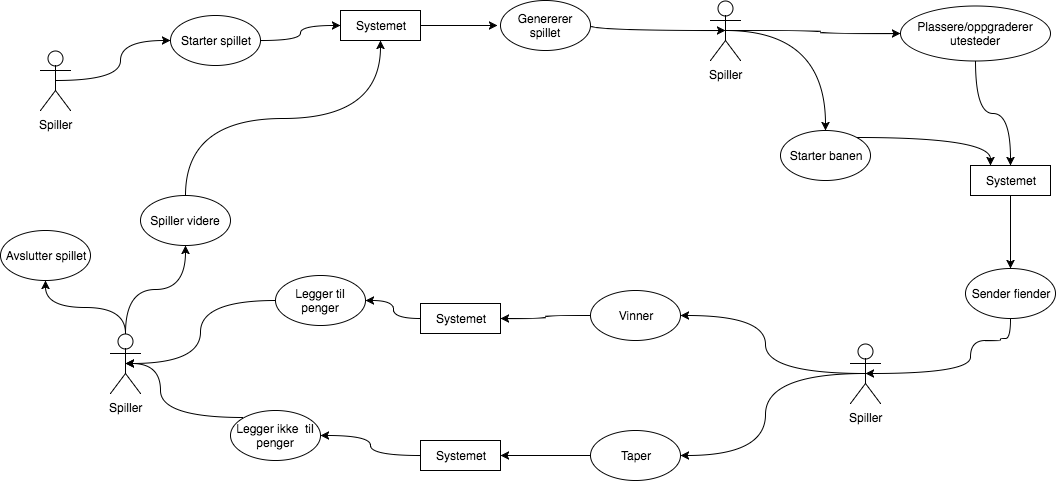
\includegraphics[width=0.98\textwidth,height=0.5\textheight]{uml.png}
%\label{uml.PNG}
figur 1:bruksmønster UML diagram
\section{Spilleregler}

\subsection{Objekt:}


Plassere tårn utenfor fiendens sti for å drepe fiendene 

Fiendene går en vei

Spiller begynner med 10 liv

Hvis fiendene går igjennom til hovedtårnet mister man liv


Fiendene blir sterkere for hver runde

Tårn må plasseres strategisk

\subsection{Poeng:}

Begynner med null poeng

Får 100 poeng for å fullføre første runde, og deretter mer for hver runde

Poengene akkumuleres og lagres som en high score

\subsection{Penger:}

 Begynner med null penger

Får penger for hver drepte fiende

Fiender av ulik styrke gir ulik mengde penger

Sterkere fiende gir mer penger

Blir brukt til å lage nye tårn eller oppgradere dem

\section{Skisse av kart og spill}


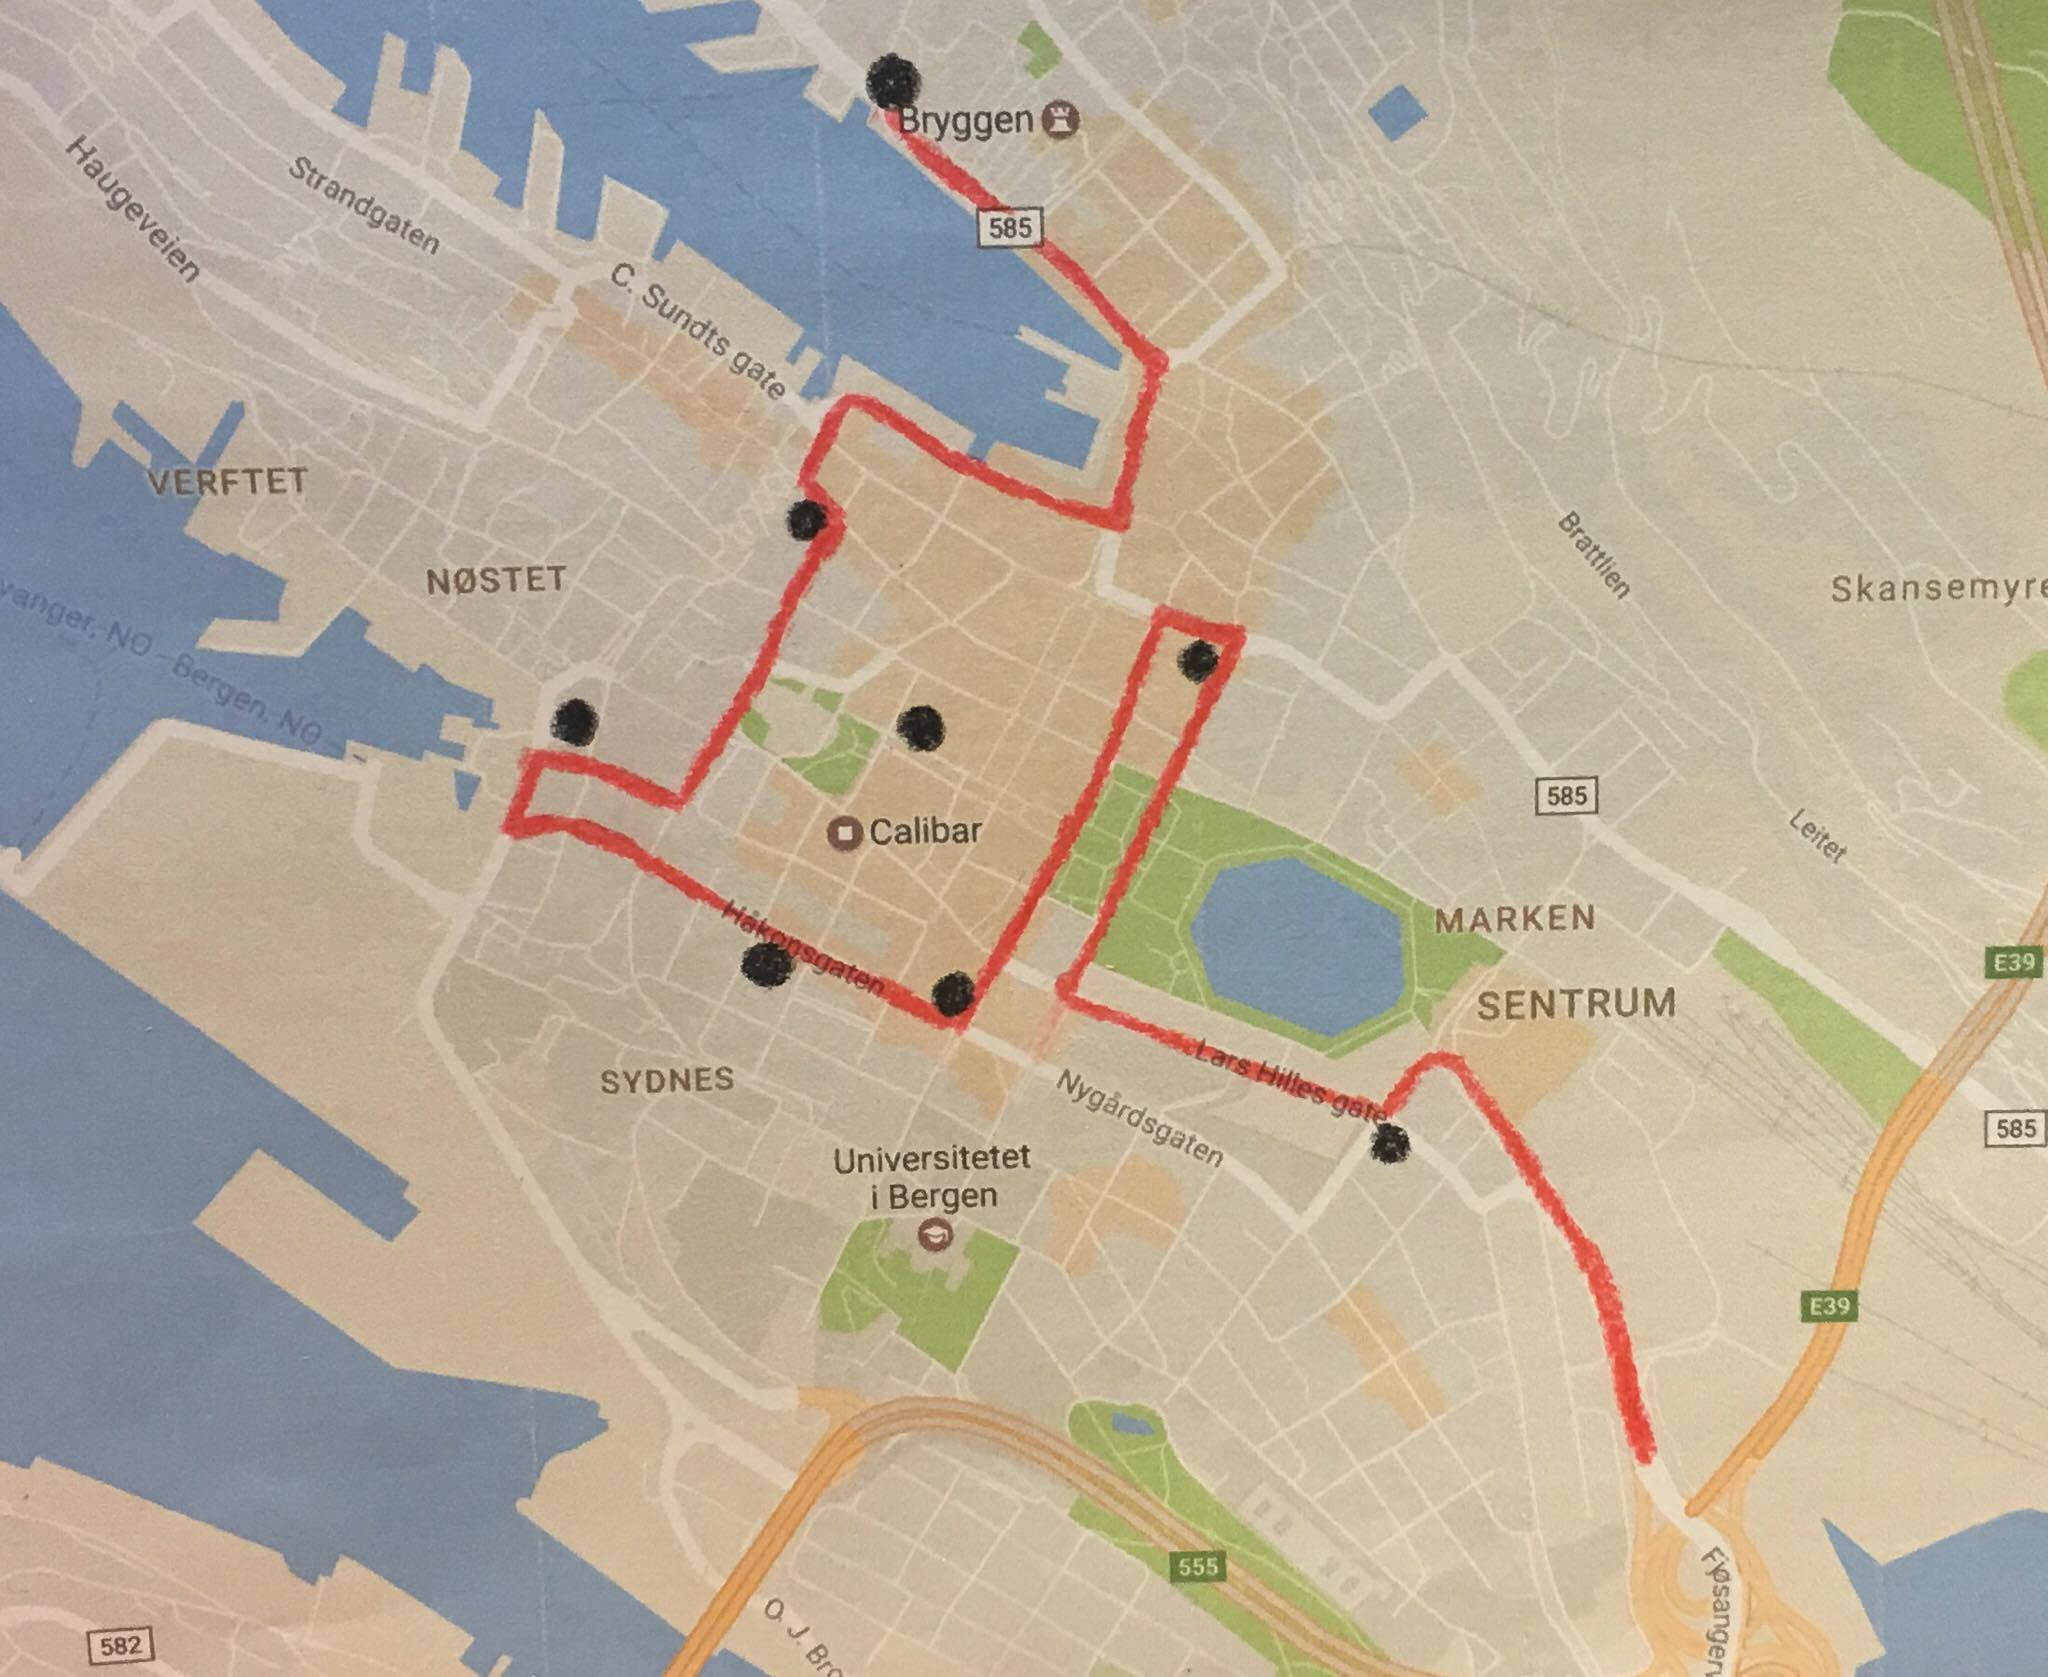
\includegraphics[width=0.98\textwidth,height=0.5\textheight]{kart.jpg}
%label{kart.jpg}

Figur 2: skisse av kart

Kartet er en røff skisse av hvordan en bane vil se ut i Bergen. 
Den røde linjen er stien som begynner ved bryggen og beveger seg rundt sentrum og til slutt til det som vil være hovedtårnet.
Svarte prikkene vil være tårn som er plassert strategisk rundt omkring på kartet.Fiendene vil gå langs stien mot hovedtårnet og tårnene som er utesteder vil da skyte alkohol mot de. 
\newpage

\section{Referat}

\subsection {Referat 1}

12:15 14 februar 2017

Alle tilstede.

Vi begynte med en god idémyldring hvor vi valgte hvilket type spill 
vi vil lage og hvilken type åpen data vi vil implementere. Deretter skrev vi en røff sketsj på hva spillet skal inneholde og hvilke ting vi vil skal implementeres i spillet.  Vi lagde også en røff sketsj på use-case text og spillereglene.

\subsection {Referat 2}

12:10 15 februar 2017

Alle tilstede.

Vi splittet opp et par av oppgavene for å øke effektiviteten. En tok ansvar for å skissere opp uml skjemaet og en skisse av banen for spillet vårt. En skrev introduksjon og begynnelsen av brukermanualen i tillegg til use case texten, og siste skrev brukerfortelling.

\subsection{ Referat 3}

12:15 21 februar 2017

Qaf006 og cli022 tilstede.

Skrev spillregler, ble ferdig med det som har blitt skrevet og begynte å føre over det som var gjort i hoveddokumentet.

\subsection{Referat 4}

12:00 22 februar 2017

Alle tilstede.

Gjorde siste finpuss og lastet opp uml skjema og en skisse av bane. Pushet opp alt til git.
\end{document}
